\documentclass[a4paper,oneside]{article}

%%%%%%%%%%%%%%%%%%%%%%%%%%%%%%%%%%%%%%%%%%%%%%%%%%%%%%%%%%%%%%%%%%%%%%%%%%%%%%%%%%%%%%%%%%%%%%%%%%%%%%%%%%%%%%%%%%%%%%%%%%%%%%%%%
%% PREAMBLE

% declare packages:

\usepackage{amsmath}
\usepackage{amsfonts,amsmath,amsthm}			% standard ams packgages
\usepackage[title,titletoc,toc]{appendix} % Appendix package. Not necessary, but it does make managing appendices easier
\usepackage{bm}										% bold maths symbols shorter definition: \bm{}
\usepackage{booktabs}							%	neat lines/rules for tables
\usepackage{eurosym} 							% neat symbols for Euro
\usepackage{float}								% allows more control over floats (figures, tables, etc.)
\usepackage{graphicx}							% for including graphics
\usepackage{lipsum} 							% insert random text (Lorem Ipsum)
\usepackage[colorlinks]{hyperref} % colorlinks colours the links instead of boxing them
\usepackage{natbib}								% references
\usepackage{setspace}							% single, 1.5, double spacing
\usepackage{url}									% like hyperref
\usepackage[euler]{textgreek}
\usepackage{rotating}
\usepackage{{xcolor}
%%%% Make some adjustments to the document

\newcommand\myworries[1]{\textcolor{red}{#1}}
% change from singlespace to onehalfspace to doublespace
%\singlespace
\onehalfspace
%\doublespace

% define title, author, etc.

\title{Cable Company Case Study}

\author{James Morgan}

\date{\today}

%% END OF PREAMBLE
%%%%%%%%%%%%%%%%%%%%%%%%%%%%%%%%%%%%%%%%%%%%%%%%%%%%%%%%%%%%%%%%%%%%%%%%%%%%%%%%%%%%%%%%%%%%%%%%%%%%%%%%%%%%%%%%%%%%%%%%%%%%%%%%%

\begin{document}

\maketitle

\begin{singlespacing} % wraps abstract to be written with single line spacing
	\begin{abstract}
		This paper focuses on the exorbitant cost and lack of quality of broadband internet access
		in the United States relative to OECD countries and the inefficient competitive
		dynamics present in the Cable Industry. More specifically, it shows that Cable Companies will
		not be able to compete in perpetuity due to innovation, inflation, higher interest rates and an
		excessive debt load. By utilizing a continuous state model of industry entry and exit, this paper
		highlights the unlikelihood that US Cable Companies will continue to have strong performance.
		Moreover, rising inflation and higher interest rates will present even stronger headwinds for
		Cable Companies. These findings will demonstrate the high social costs created by the Cable
		Companies and present a call to action for entrepreneurs and regulatory authorities.\end{abstract}
	\end{singlespacing}
\pagebreak

\section{Introduction}
	\:\:\:\:\:\: The shift to remote work has increased the need for network connectivity and is
	beginning to commoditize network services. Consequently, federal and state agencies have taken an interest in the industry. 
	For example, President Joe Biden signed an executive order on November 15, 2021 to allocate about \$ 65 billion to increase 
	broadband penetration and make broadband more affordable for lower-income households across the United States. 
	Moreover, alternative conduits for broadband connection present a market ripe for disruption through innovation. For example, Elon Musk's company Starlink may
	be able to offer more affordable internet access to customers in rural areas. Starlink uses
	advanced satellites in a low orbit to provide low latency broadband internet access across the
	globe. The development and implementation of 5G may further dampen Cable Company profits,
	especially since 20\% of Americans are smart phone only users. (Bandyopadhyay et al. 2020)

	The looming threat of an economic downturn is yet another headwind for Cable
	Companies. The CPI was up 5.4\% year over year in September and the threat of high long term
	inflation is very real. The COVID-19 pandemic and associated government support has created
	an extremely tight labor market. According to the NFIB, 51\% of small business owners reported
	job openings they could not fill in September 2021. This is a record high and is up one point
	from the previous month. (“Jobs Report and Jobs Data from the NFIB Small Business Research
	Center”, n.d.) It seems likely that the FED's hand will be forced and interest rates will rise as a
	function of inflation.

	The relative cost and quality of broadband internet access in the United States poses
	serious concerns about the efficacy of the industry model. The bar graph from the OECD
	Broadband Portal below indicates that the United States is behind many competitors regarding
	broadband internet penetration. This is surprising given the United States overall economic
	presence and brings to the light pressing need to increase penetration rates.

	The success of the Rural Electrification Act of 1936 demonstrates the tremendous social benefits of electrification. 
	\myworries{/*NEEDS REA FACTS*/}
	The corresponding plot below plots energy consumption by income per capita which illustrates a strong positive correlation between energy consumption and income per capita. 
	Therefore, the success of the rural electrification act is plain and clear due to its high ROI and the strong positive correlation between energy consumption and income per capita. 
	\begin{figure}
		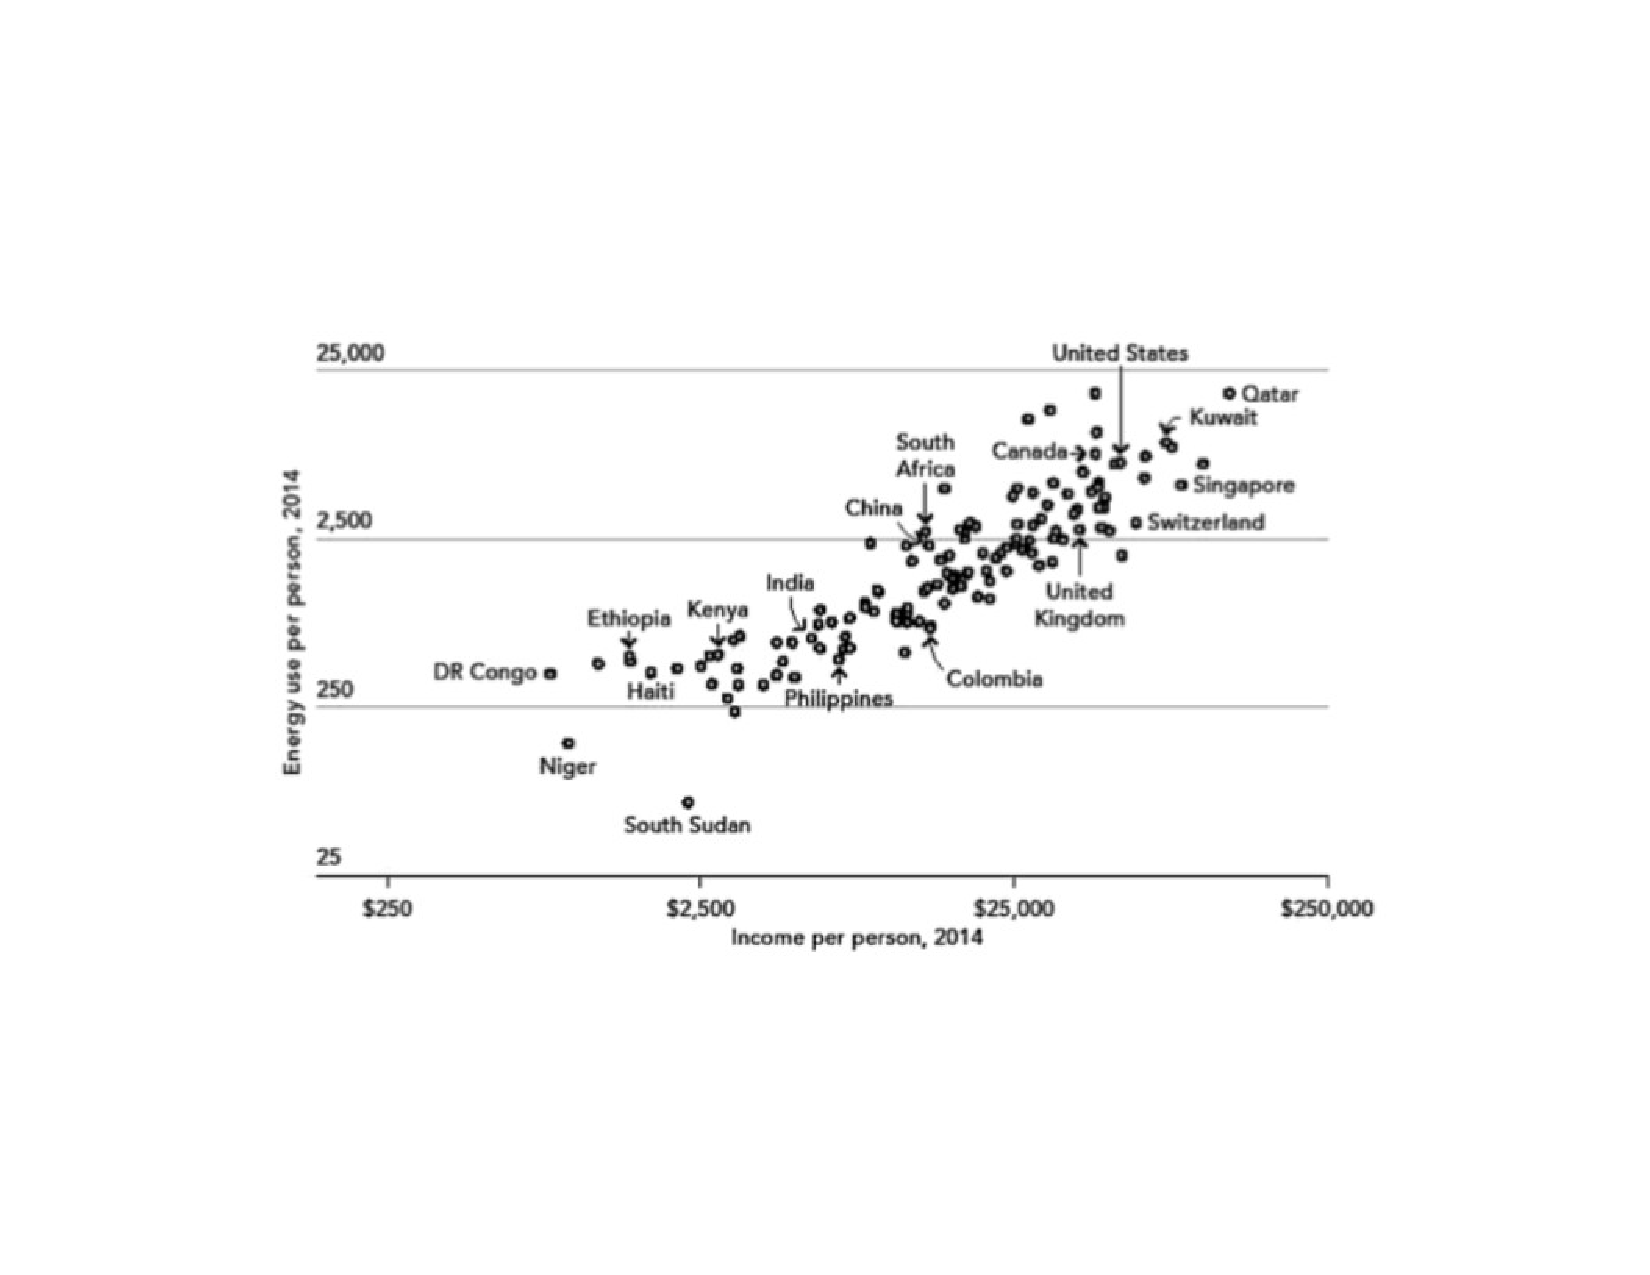
\includegraphics[width=\columnwidth]{img/GATES}
		\caption{Gates, B. (2021). How to avoid a climate disaster. Allen Lane.}
	\end{figure}

	When Joe Biden announced the American Jobs Plan in March of 2021, he asserted that “Broadband internet is the new electricity. 
	It is necessary for Americans to do their jobs, to participate equally in school learning, health care, and to stay connected.” 
	This demonstrates that broadband internet access is a necessity and, therefore, a commodity. 
	Therefore it is imperative that the competitive dynamics of the broadband industry maximize social benefits.

\section{Literature Review}

\:\:\:\:\:\:The inspiration for this paper arises from the success of the Rural Electrification Act which provided low-interest loans in the 1930s to cooperatives to lay distribution lines to farms and aid in wiring homes. 
Kitchens and Fishback found that the number of electrified rural homes doubled in the United States within five years of the program's beginning. 
Their work suggets that REA loans contributed significantly to increases in crop output and productivity. 
Similarly, Tim Sablak notes that virtually all rural Americans had access to power within a 20- to 25-year period of the program's inception. 
In addition, almost all REA loans were repaid given that the default rate was less than 1 percent.

The expansion of broadband internet access strongly resembles the deployment of electricity in the 1920s.
The digital divide that deprvies rural Americans adequate access to broadband internet closely parallels the digital divide present in electricity deployment 100 years ago.
The private markets failed to provide an adequate incentive in rural areas for both industries. Nonetheless, both sectors witnessed tremendous growth. 
By 1929, five holding companies controlled 80 percent of the electrical generating capacity of the nation. 
The electrical industry grew by 244 percent, from \$ 882 million in 1920 to \$ 2155 million in 1929. \myworries{PLEASE INCLUDE INFORMATION ABOUT ISP MONOPOLIES}
Similarly, the five key industry players in the broadband industry (Altice USA, Cable One, Charter Communications, Comcast and Cox Communications) have averaged a 25 percent return on invested capital.  
While broadband internet service providers are not as consolidated as electric companies, they certainly exert tremendous monopoly power through regional monopolies as indicated by Ferguson's “The U.S. Broadband Problem”, Krugman's “Barons of Broadband” and many others.

One key issue with existing economic literature is that it is very difficult to pinpoint how monopolistic internet service providers are creating social costs. 
Using a fixed-effect disequilibrium broadband penetration model and OECD country broadband subscription data, W.J. Mayer et al, concluded that broadband markets are potentially (likely) in disequilibrium. 
Similarly, Gruber and Koutroumpis conducted an analysis of different regulatory interventions on broadband diffusion. 
Their findings assert that reducing market power of incumbents increases the speed of broadband diffusion. 
However, the results also find that the diffusion effect from regulatory access dissipates after 3-4 years. 
Moreover, it does not take into account the quality of broadband access. 

The government policy responses to promote competition amongst network providers have been ineffective so far. 
Pindyk challenged the efficacy of the Telecommunications Act of 1996 citing that it discouraged investment. 
More specifically, by forcing incumbents to share their network capital with new entrants, new investment is deterred by uncertainty of future demand at the entry price. 
Despite this, some empirical evidence suggests that this is not the case for all circumstances. 
More specifically, there is evidence to support that an appropriately specified access price can reduce social costs.
Nonetheless, political uncertainty remains.

Broadband internet industry dynamics are highly uncertain due to innovation, regulatory risks and economic uncertainty. 
Meijer et al. touch on the technological uncertainties created by the characteristics of new technology, adaptations to infrastructure and alternative technologies. 
Pindyck demonstrates that the population tends to grow steadily, however, the willingness to purchase internet services varies greatly. 
Furthermore, the opportunity cost of capital in a telecommunications investment is increased by 70\% because investment reversibility is virtually impossible.
The concept of uncertainty is often left out of traditional models of entry and exit. Dixit asserts that the most important feature of entry and exit is “hysteresis”: the failure of an effect to reverse itself as its underlying cause is reversed. 

\section{Data}

\:\:\:\:\:\: The primary dataset for this project comes from the 2021 third quarter Charter Communications trending schedule.~\citep{chtr_rep} 
Charter Communications' business model is more focused on broadband internet and is, consequently, more suitable for this project.
Only revenues attributed to internet service are included in the project dataset. 
Furthermore, costs and expenses that are explicitly used for non-internet related activities are removed from the dataset.
In an abundance of caution, any costs and services that relate to internet services are included in the final dataset. 
It is assumed that these cost and expenses are required operating expenses for a purely broadband internet service company.
The final dataset is adjusted to a per customer level so that the model can test for markets of different sizes.
Additional information about financial calcuations is provided in the appendix.

\section{Models}
\subsection{Optimal Monetary Policy Model}

\:\:\:\:\:\:\:\:Consider a monetary authority who wishes to control the nominal interest rate  \emph{x} to minimize the variation of the inflation rate s\textsubscript{1} + the GDP gap s\textsubscript{2} around specified targets s\textsuperscript{*}\textsubscript{1} and s\textsuperscript{*}\textsubscript{1}.

\begin{equation}
	L(s) = 0.5(s-s^{*})^{T}\Omega(s-s^{*})
	\label{eq:mye1}
\end{equation} 
The corresponding state transition function is: 

\begin{equation}
	g(s,x,\epsilon) = \alpha + \beta \gamma x + \epsilon
	\label{eq:myeq2}
\end{equation} 

\begin{equation*}
s \subseteq \mathbb{R}^{2} \:\:\:	
x \subseteq [0, \infty)
\end{equation*}

Where s is a 2x1 vector containing the inflation rate and the GDP gap, s* is a 2x1 vector of targets, and Ω is a 2 x 2 constant positive definite matrix of preference weights. 
\begin{equation*} % stars * suppress labels / numbers appearing
	\bm{s^{*}} = 
		\left.
			\begin{bmatrix}
				0	\\
				1	\\
			\end{bmatrix}
		\right.
	\bm{\Omega} = 
		\left.
			\begin{bmatrix}
				0.3	&	0.0\\
				0.0	&	1.0\\
			\end{bmatrix}
		\right.
\end{equation*}

Assume that the inflation rate and the GDP gap are a joint controlled exogenous linear Markov process.

\begin{equation}
	s_{t+1}= \alpha+\beta s_{t}+\gamma x_{t}+\epsilon_{t+1} 
	\label{eq:mye3}
\end{equation}

Where \textalpha \: and \textGamma \: are 2 × 1 constant vectors, \textbeta \: is a 2 × 2 constant matrix, and \textepsilon \: is a 2 × 1 random vector with zero mean. 

\begin{equation*}
	\bm{\alpha} =
		\left.
			\begin{bmatrix}
				0.3	&	0.0\\
				0.0	&	1.0\\
			\end{bmatrix} 
		\right.
	\bm{\beta} =      
		\left.
			\begin{bmatrix}
				0.3	&	0.0\\
				0.0	&	1.0\\
			\end{bmatrix} 
		\right.
	\bm{\Gamma} =
		\left.
			\begin{bmatrix}
				0	\\
				1	\\
			\end{bmatrix}
		\right.
	\bm{\epsilon} = 
		\left.
			\begin{bmatrix}
				0.04 &	0.00\\
				0.00 &	0.04\\
			\end{bmatrix}
		\right.
\end{equation*}

  To formulate as a maximization problem, posit reward function equaling negative loss function
  \begin{equation*}
	  f(s, x) = -L(s)
  \end{equation*}
  
  The sum of current and expected future rewards satisfies the Bellman equation.
  \begin{equation}
	  V(s) = \max\limits_{0 \leq x }{-L(s)\epsilonV(g(s,x,\epsilon))}
	  \label{eq:myeq3}
  \end{equation}
  
  Given the model structure, one cannot omit the possibility that x <=0 will bind in certain states.
  Therefore, the shadow-price function λ(s) characterized by Euler conditions:
  \begin{equation}
	  \delta \lambda^{T} E_{\epsilon} (g(s, x, \epsilon)) =  \mu
  \end{equation*}
  \begin{equation}
	  \lambda(s) = -\Omega(s_{t}-s^{*}) + \delta \beta^{T}E_{\epsilon} \lambda (g(s,x,\epsilon))
  \end{equation*}
  
  The Shadow price function represents the value of the Lagrange multiplier. Therefore, in the context of this problem, the shadow price function is the change in the optimal value per unit of infinitesimal change in the constraints (nominal interest rate and inflation variation). 
  
  It follows that along the optimal path
  \begin{equation}
	  \delta \gamma TE_{t} \lambda_{t+1} = \mu_{t}
  \end{equation}
  \begin{equation}
	  \lambda_{t} = -\omega(s_{t}-s^{*})+\delta \beta^{T}E_{t} \lambda_{t}+1
  \end{equation}
  \begin{equation*}
	x_{t}\geq 0 \mu_{t} \leq 0 x_{t}>0 ==> u_{t} - 0
  \end{equation*}
  Thus, in any period, nominal interest rate x is reduced until either the long-run marginal reward  µ or the nominal interest rate is driven to zero. 

\subsection{Profit Model}

\subsubsection{Standard Profit Equation}
\:\:\:\:\:\: Consider a profit model for a cable company that is defined by internet revenue per passing less two costs bases: \emph{C\textsubscript{f}} and \emph{C\textsubscript{v}}. 
\emph{C\textsubscript{f}} represents the fixed average customer per customer and \emph{C\textsubscript{v}} represents the variable average cost per customer. 
Additional information about financial calcuations is provided in the appendix. 
\begin{equation}
	\pi_{t} = \emph{rev} * \emph{pen} - (C_{f}+C_{v})
\end{equation}
This equation represents the short run profit per quarter. 
Due to significantly high fixed costs, \emph{C\textsubscript{f}} is to be paid each period and theoretically, represents required interest payments.

Now consider a new cable company entering the market at time t\textsubscript{new}:
\begin{equation}
	\pi_{t_{new}} = \emph{rev} * \emph{pen} - (C_{f}+C_{v})
\end{equation}
Assuming all else equal, the fixed cost for the new cable company is adjusted to the new interest rate.

\subsubsection{Demand Equation}
\:\:\:\:\:\:Now consider a demand function that defines a functional relationship between penetration rate and cost to customer per passing.
Let Q equal estimated passings (the estimated number of customers that it can provide services for).
Let C be the per-acre variable costs of operation (C) which are known and constant.
\begin{equation}
	P = Y - bQ
\end{equation}
	Where Y is the stochastic variable and \emph{b} is the constant slope. The variable Y follows a geometric Brownian motion represented by:
\begin{equation}
	dY = \alpha Y dt + \sigma Y dz
\end{equation}
	\textalpha\:\: is the drift parameter or in other words, the growth rate of Y, \textsigma \:\: is the standard deviation in the drift, and dz the increment of the Weiner process.

\subsubsection{Short Run Profit Model for Entry and Exit}
\:\:\:\:\:\:	Estimated passings are determined by the stock of capital and \myworries{INTEREST RATE ENVIRONMENT},
	Q = G(K); \:\:\:\:\:\: Q \textgreater G'(K); \:\:\:\:\:\: Q \textless G'(K);
	Therefore, the profit of the firm is given by:

\begin{equation}
	\pi = [Y - bG(k)-C]G(K)
\end{equation}
\subsubsection{Entry and Exit Strategies}
	The model herein is an expansion of the models of Dixit (1989) and Dixit and Pindyck (1994). 
The expansion was created by lsik (2003) for Agricultural Economics, however, it is generally applicable to the network service provider industry.
\begin{equation}
	\begin{split}
		-A(Y^O_H)^{\beta_1} + B(Y^O_H)^{\beta_2}  + G(K_0) \times \bigg( \frac{Y^O_H}{\emph{p}-\alpha} -  \frac{bG{K}+C}{\emph{p}}    \bigg) =K_0 
		\\
		\\
		-\beta_1 A (Y^O_H)^{\beta_1-1} + -\beta_2 B (Y^O_H)^{\beta_2-1}  + \frac{G(K_0)}{\emph{p}-\alpha} = 0 
		\\
		\\
		-A(Y^O_L)^{\beta_1} + B(Y^O_L)^{\beta_2} + G(K_0) \times \bigg( \frac{Y^O_L}{\emph{p}-\alpha} -  \frac{bG{K_0}+C}{\emph{p}}    \bigg) = -E
		\\
		\\
		-\beta_1 A (Y^O_L)^{\beta_1-1} + -\beta_2 B (Y^O_L)^{\beta_2-1}  + \frac{G(K_0)}{\emph{p}-\alpha} = 0
	\end{split}
\end{equation}
Where B and A are constants to be determined, Y\textsuperscript{O}\textsubscript{H}
\cite{Cap_Choice}
\section{Results}\label{sec:res}
	\section{Conclusion}
\bibliographystyle{ecca}
	\bibliography{myrefs}
\begin{appendices}

\pagebreak	
\section{More on data}\label{app:dat}
\pagebreak
\begin{table}%[ht] or say [H]
	\centering
	\begin{tabular}{cccccc}\hline % each column is centered (else could have left aligned [l] or right [r])
		\toprule			
		Label & Q1 2019 & Q2 2019 & Q3 2019 & Q4 2019 & FY 2019 \\
		\midrule
		Penetration Rate & 50\% & 50\% & 51\% & 51\% & 51\% \\
		\:\: Revenue per Passing & $78.31 & $79.49 & $80.77 & $83.31 & $319.57 \\
		\:\: Cost to Service Customer Per Capita & $35.46 & $34.23 & $36.47 & $34.40 & $139.53 \\
		\:\: Other Costs Per Passing & $43.34 & $41.84 & $44.57 & $42.04 & $170.54 \\
		\bottomrule
	\end{tabular}
	\caption{Data points for 2019}
	\label{tab:myt1}
\end{table}
\begin{table}%[ht] or say [H]
	\centering
	\begin{tabular}{cccccc}\hline % each column is centered (else could have left aligned [l] or right [r])
		\toprule			
		Label & Q1 2020 & Q2 2020 & Q3 2020 & Q4 2020 & FY 2020 \\
		\midrule
		Penetration Rate & 52\% & 53\% & 54\% & 54\% & 54\% \\
		\:\: Revenue per Passing & $84.07 & $85.94 & $89.06 & $91.22 & $347.49 \\
		\:\: Cost to Service Customer Per Capita & $35.26 & $35.06 & $35.87 & $35.16 & $140.19 \\
		\:\: Other Costs Per Passing & $43.09 & $42.85 & $43.84 & $42.97 & $171.34 \\
		\bottomrule
	\end{tabular}
	\caption{Data points for 2020}
	\label{tab:myt1}
\end{table}
\begin{table}%[ht] or say [H]
	\centering
	\begin{tabular}{cccccc}\hline % each column is centered (else could have left aligned [l] or right [r])
		\toprule			
		Label & Q1 2021 & Q2 2021 & Q3 2021 \\
		\midrule
		Penetration Rate & 55\% & 55\% & 55\% \\
		\:\: Revenue per Passing & $94.90 & $96.89 & $99.04 \\
		\:\: Cost to Service Customer Per Capita & $33.66 & $33.91 & $35.07 \\
		\:\: Other Costs Per Passing & $41.14 & $41.44 & $42.86 \\
		\bottomrule
	\end{tabular}
	\caption{Data points for 2021}
	\label{tab:myt1}
\end{table}

\section{Figures}\label{app:figures}

\begin{figure}
	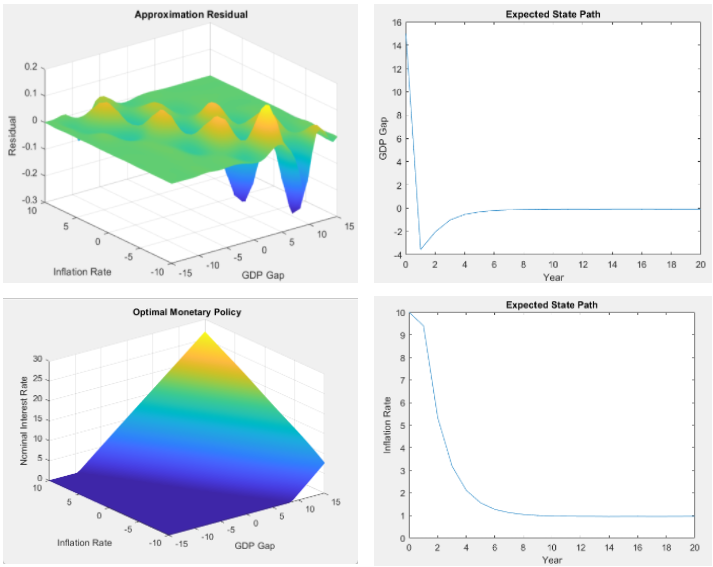
\includegraphics[width=\columnwidth]{img/Optimal_Monetary_Policy/Optimal_Monetary_Policy}
	\caption{Approximation Residuals}
	\label{fig:myf1}
\end{figure}
\begin{figure}
	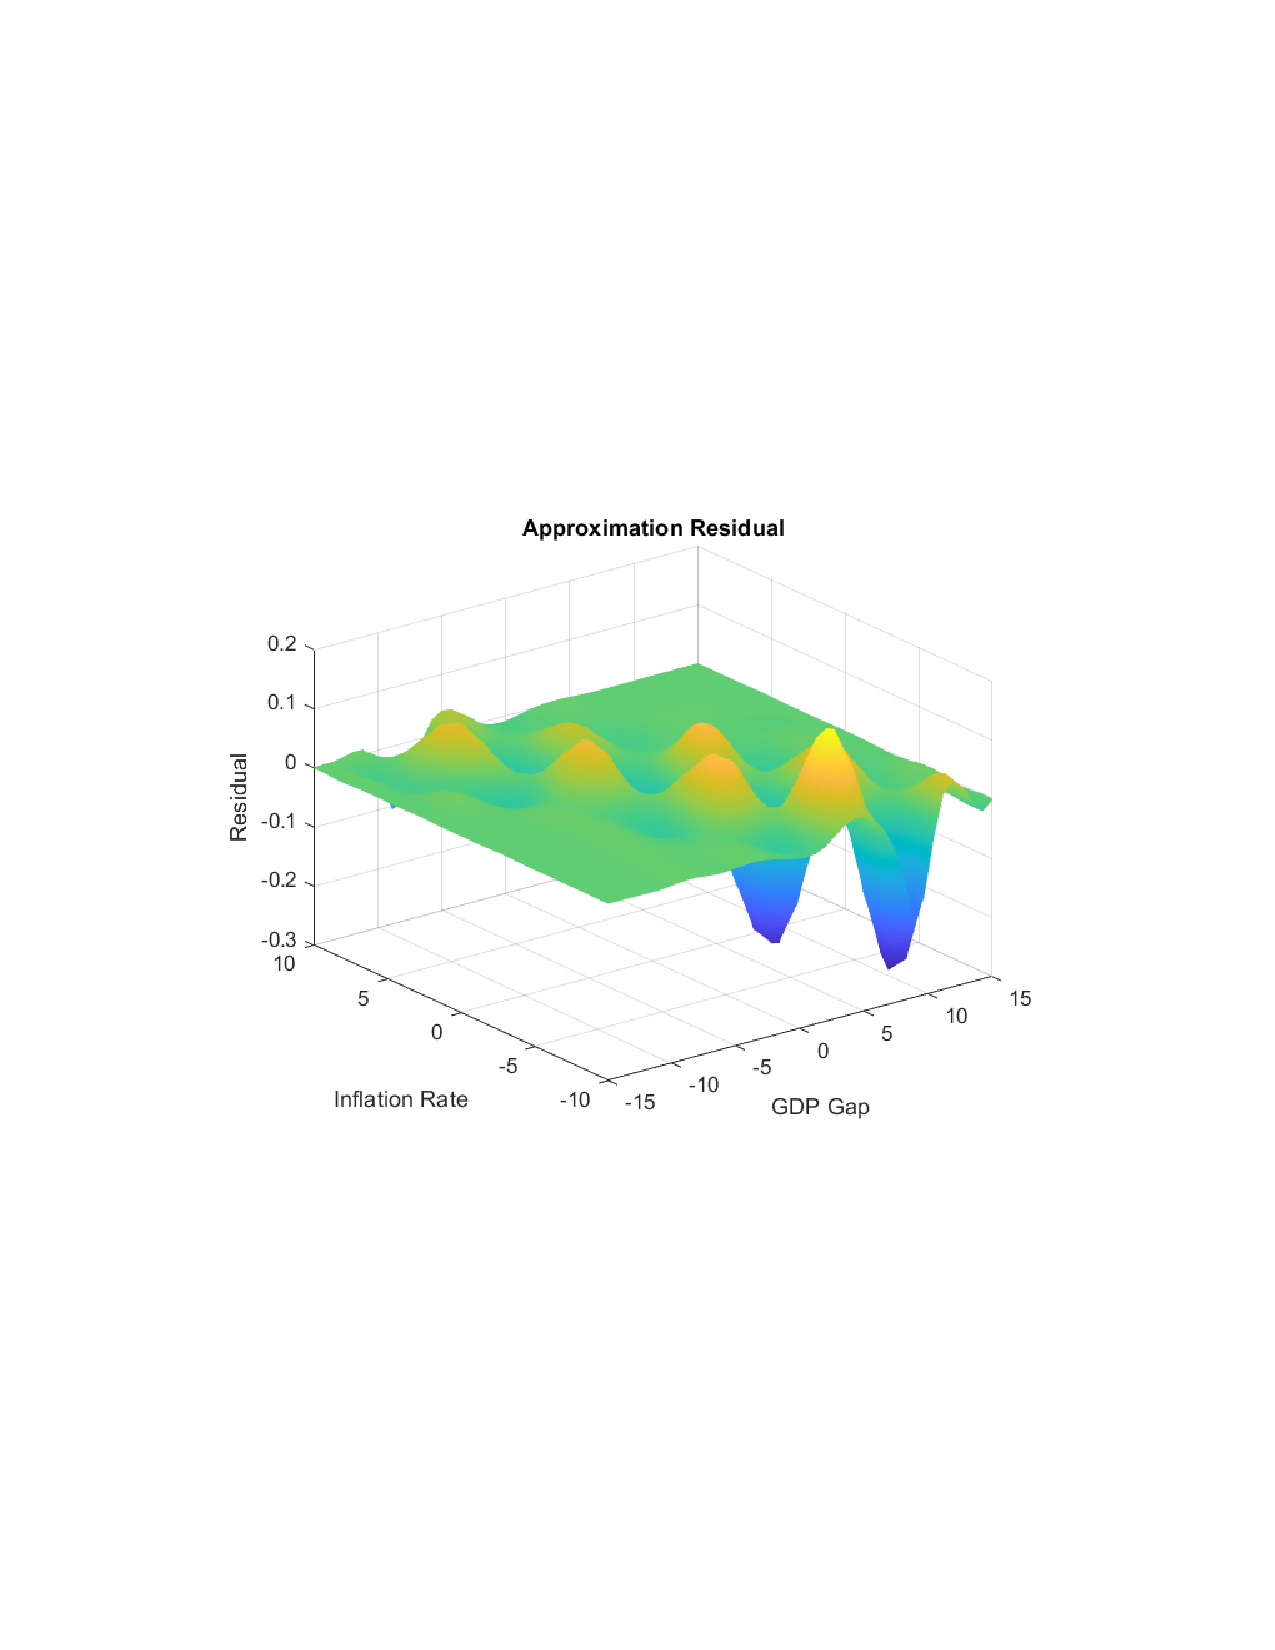
\includegraphics[width=\columnwidth]{img/Optimal_Monetary_Policy/Approximation_Residual}
	\caption{Approximation Residuals}
	\label{fig:myf2}
\end{figure}
\begin{figure}
	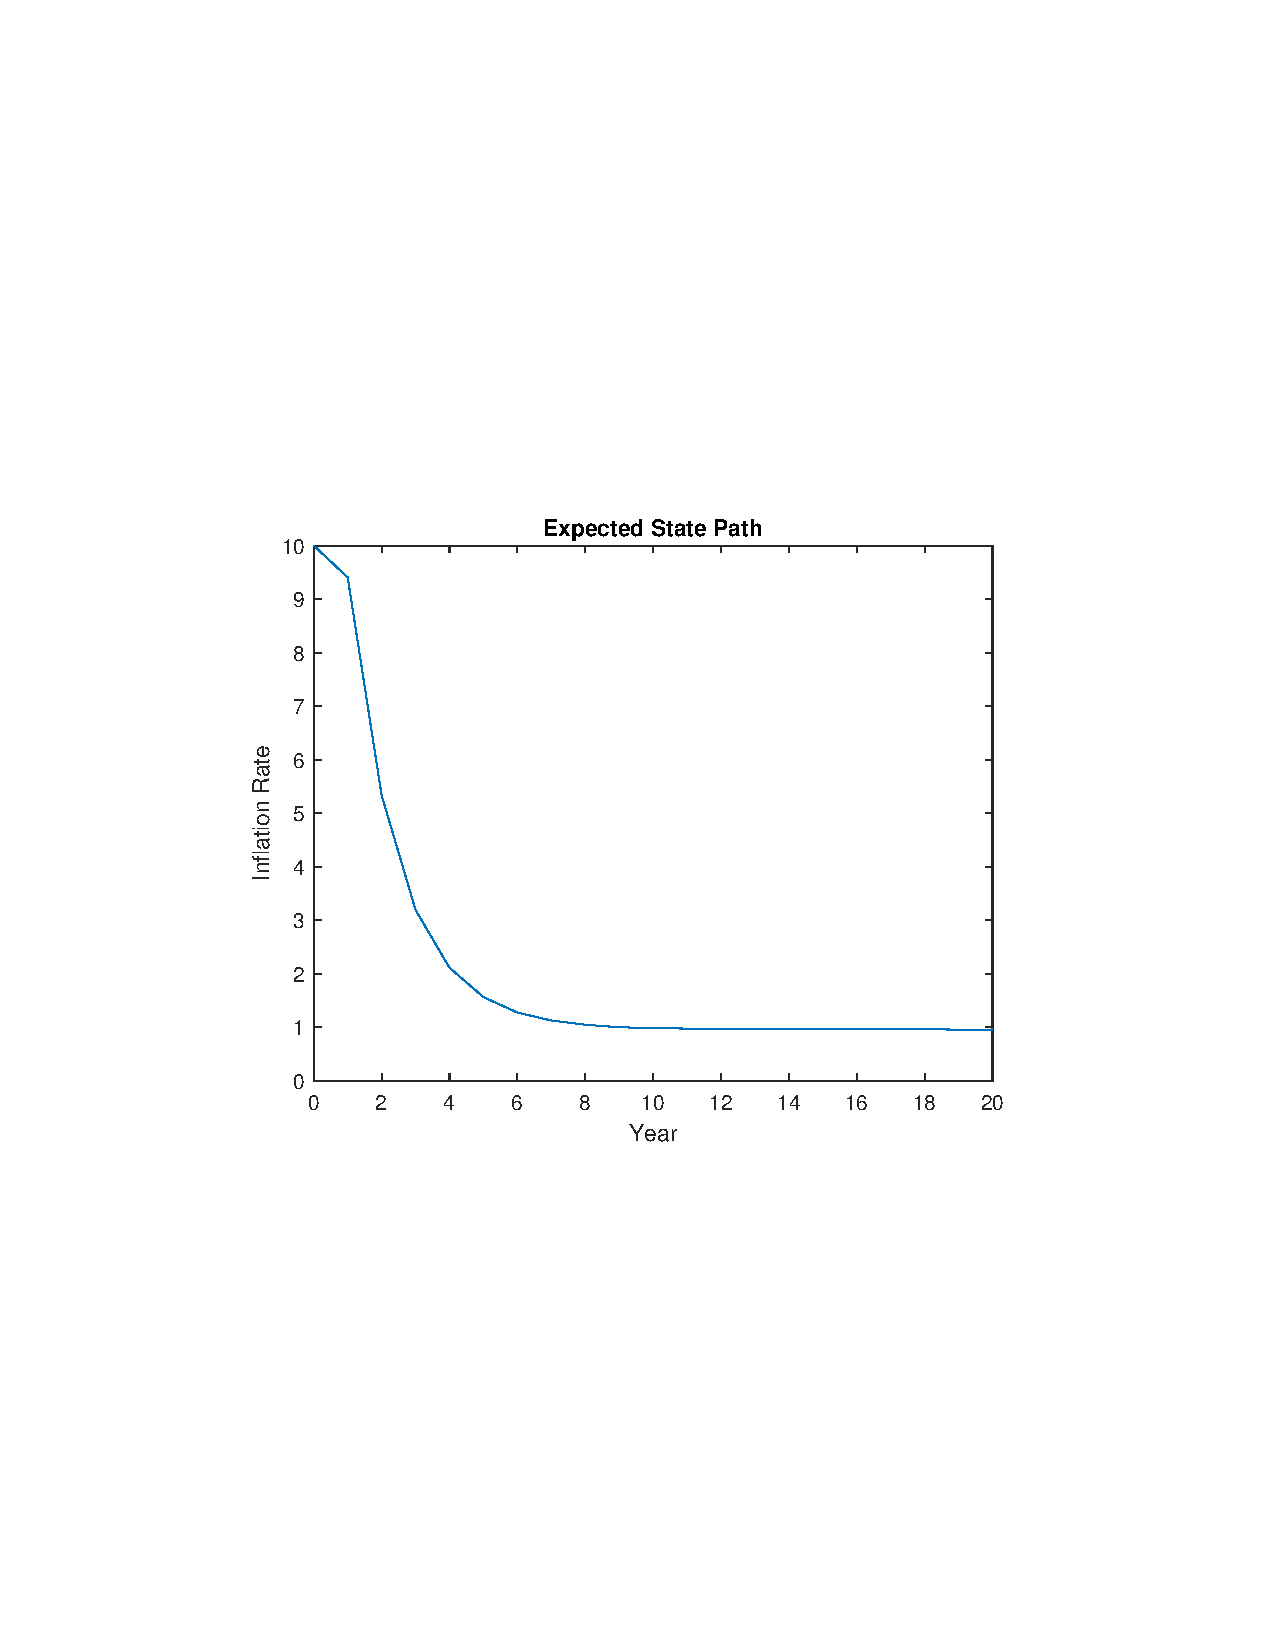
\includegraphics[width=\columnwidth]{img/Optimal_Monetary_Policy/Expected_State_Path_InflationRate}
	\caption{Approximation Residuals}
	\label{fig:myf3}
\end{figure}
\begin{figure}
	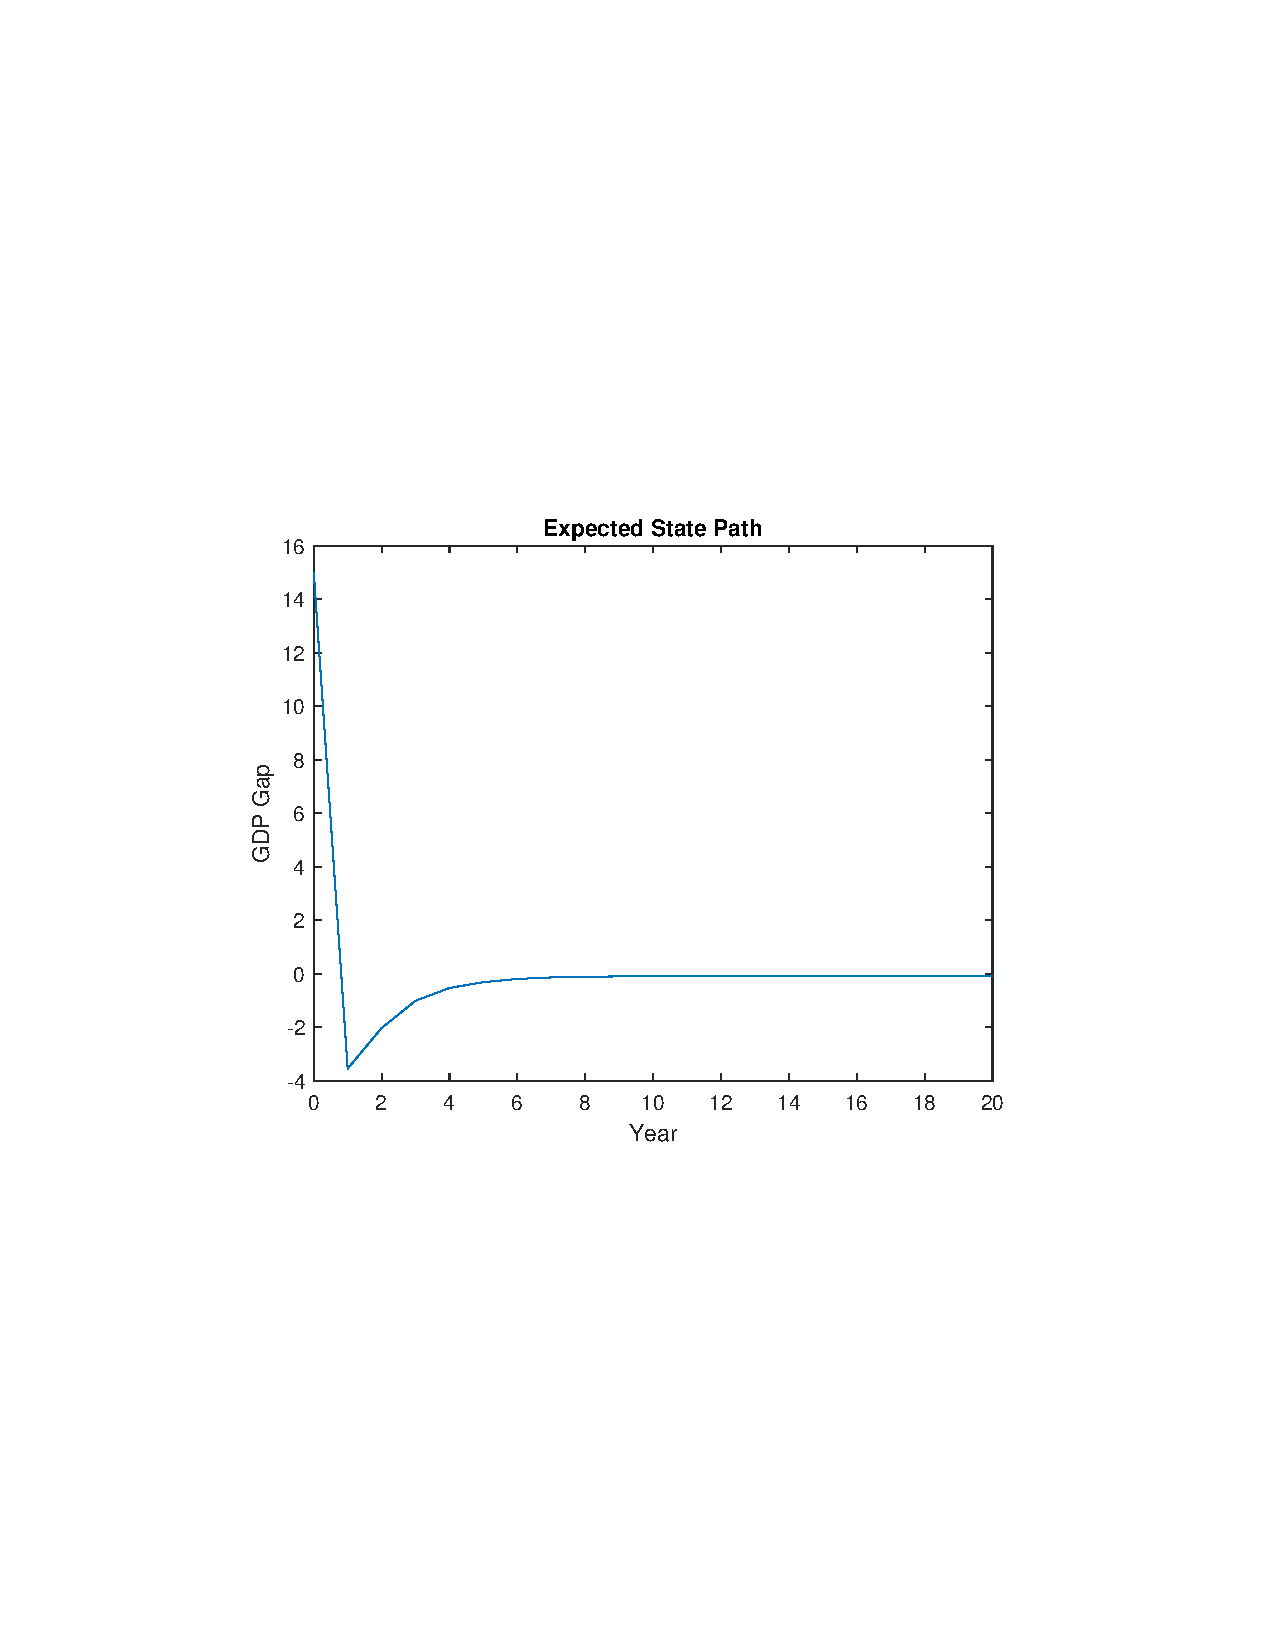
\includegraphics[width=\columnwidth]{img/Optimal_Monetary_Policy/Expected_State_Path_GDP_GAP}
	\caption{Approximation Residuals}
	\label{fig:myf4}
\end{figure}

\pagebreak
\bibliographystyle{ecca}
\bibliography{newrefs}

\end{appendices}
\end{document}